\chapter{The burning process in graphs}\label{chapter:graph-burning-examples}

\section{Burning a simple path or cycle}\label{section:burn-path}

A path is simple to burn. A path and a cycle (of equal length) are equivalent from the burning perspective. In each step, we select one new unburnt ``victim'' vertex (a fire source) and burn vertices adjacent to other clusters. This follows from the definition of graph burning that we discussed in \Cref{section:burning-intro}. Each cluster burns its neighbour vertices and includes them in itself. The interesting fact here is, a burning cluster can spread fire to atmost two more vertices. Each burning cluster starts with on single vertex (a fire source) and in successive time steps, it can get enlarged in size by atmost two more vertices. A newly burned fire source also acts as a distinct cluster.

\subsection{Burning a path (or a cycle) of infinite length}

\index{burning simple path or cycle} Let us consider that a path is so long (of infinite length) that we can put fire sources in such a way that any two fire sources are at infinite distance from one another, as shown in \Cref{figure:burn-path-inf}. We select a fire source, and the fire in all other clusters spreads to their respective neighbouring vertices, i.e., each burning cluster has $2$ more vertices; this is shown in \Cref{table:burn-path-inf}.

\begin{figure}
    \begin{minipage}{1\textwidth}
        \centering
        \subfigure[]{
            \begin{tikzpicture}
                \draw[dashed] (0,0) -- (1,0);
                \draw(1,0) -- (4,0);
                \draw(4,0) -- (4,2);
                \draw(4,2) -- (0,2);
                \draw(0,2) -- (0,4);
                \draw(0,4) -- (3,4);
                \draw[dashed] (3,4) -- (4,4);
                
                \node [label=below:{original path \textit{(step 0)}}] (BA) at (2,0) {};
            \end{tikzpicture}
        }
        \subfigure[]{
            \begin{tikzpicture}
                \draw[dashed] (0,0) -- (1,0);
                \draw(1,0) -- (4,0);
                \draw(4,0) -- (4,2);
                \draw(4,2) -- (0,2);
                \draw(0,2) -- (0,4);
                \draw(0,4) -- (3,4);
                \draw[dashed] (3,4) -- (4,4);
                
                \node [circle, draw=black, fill=black, inner sep=1pt, minimum size=5pt, label=below:{$1a$}] (BA) at (2.5,0) {};
            \end{tikzpicture}
        }
        \subfigure[]{
            \begin{tikzpicture}
                \draw[dashed] (0,0) -- (1,0);
                \draw(1,0) -- (4,0);
                \draw(4,0) -- (4,2);
                \draw(4,2) -- (0,2);
                \draw(0,2) -- (0,4);
                \draw(0,4) -- (3,4);
                \draw[dashed] (3,4) -- (4,4);
                
                \node [circle, draw=black, fill=black, inner sep=1pt, minimum size=5pt, label=below:{$1a$}] (BA) at (2.5,0) {};
                \node [circle, draw=black, fill=black, inner sep=1pt, minimum size=2pt, label=below:{}] (BA) at (2.25,0) {};
                \node [circle, draw=black, fill=black, inner sep=1pt, minimum size=2pt, label=below:{}] (BA) at (2.75,0) {};
                
                \node [circle, draw=black, fill=black, inner sep=1pt, minimum size=5pt, label=below:{$2a$}] (BA) at (2,2) {};
            \end{tikzpicture}
        }
        \subfigure[]{
            \begin{tikzpicture}
                \draw[dashed] (0,0) -- (1,0);
                \draw(1,0) -- (4,0);
                \draw(4,0) -- (4,2);
                \draw(4,2) -- (0,2);
                \draw(0,2) -- (0,4);
                \draw(0,4) -- (3,4);
                \draw[dashed] (3,4) -- (4,4);
                
                \node [circle, draw=black, fill=black, inner sep=1pt, minimum size=5pt, label=below:{$1a$}] (BA) at (2.5,0) {};
                \node [circle, draw=black, fill=black, inner sep=1pt, minimum size=2pt, label=below:{}] (BA) at (2,0) {};
                \node [circle, draw=black, fill=black, inner sep=1pt, minimum size=2pt, label=below:{}] (BA) at (2.25,0) {};
                \node [circle, draw=black, fill=black, inner sep=1pt, minimum size=2pt, label=below:{}] (BA) at (2.75,0) {};
                \node [circle, draw=black, fill=black, inner sep=1pt, minimum size=2pt, label=below:{}] (BA) at (3,0) {};
                
                \node [circle, draw=black, fill=black, inner sep=1pt, minimum size=5pt, label=below:{$2a$}] (BA) at (2,2) {};
                \node [circle, draw=black, fill=black, inner sep=1pt, minimum size=3pt, label=below:{}] (BA) at (1.75,2) {};
                \node [circle, draw=black, fill=black, inner sep=1pt, minimum size=3pt, label=below:{}] (BA) at (2.25,2) {};
                
                \node [circle, draw=black, fill=black, inner sep=1pt, minimum size=5pt, label=left:{$3a$}] (BA) at (0,3) {};
            \end{tikzpicture}
        }
        \subfigure[]{
            \begin{tikzpicture}
                \draw[dashed] (0,0) -- (1,0);
                \draw(1,0) -- (4,0);
                \draw(4,0) -- (4,2);
                \draw(4,2) -- (0,2);
                \draw(0,2) -- (0,4);
                \draw(0,4) -- (3,4);
                \draw[dashed] (3,4) -- (4,4);
                
                \node [circle, draw=black, fill=black, inner sep=1pt, minimum size=5pt, label=below:{$1a$}] (BA) at (2.5,0) {};
                \node [circle, draw=black, fill=black, inner sep=1pt, minimum size=2pt, label=below:{}] (BA) at (1.75,0) {};
                \node [circle, draw=black, fill=black, inner sep=1pt, minimum size=2pt, label=below:{}] (BA) at (2,0) {};
                \node [circle, draw=black, fill=black, inner sep=1pt, minimum size=2pt, label=below:{}] (BA) at (2.25,0) {};
                \node [circle, draw=black, fill=black, inner sep=1pt, minimum size=2pt, label=below:{}] (BA) at (2.75,0) {};
                \node [circle, draw=black, fill=black, inner sep=1pt, minimum size=2pt, label=below:{}] (BA) at (3,0) {};
                \node [circle, draw=black, fill=black, inner sep=1pt, minimum size=2pt, label=below:{}] (BA) at (3.25,0) {};
                
                \node [circle, draw=black, fill=black, inner sep=1pt, minimum size=5pt, label=below:{$2a$}] (BA) at (2,2) {};
                \node [circle, draw=black, fill=black, inner sep=1pt, minimum size=3pt, label=below:{}] (BA) at (1.5,2) {};
                \node [circle, draw=black, fill=black, inner sep=1pt, minimum size=3pt, label=below:{}] (BA) at (1.75,2) {};
                \node [circle, draw=black, fill=black, inner sep=1pt, minimum size=3pt, label=below:{}] (BA) at (2.25,2) {};
                \node [circle, draw=black, fill=black, inner sep=1pt, minimum size=3pt, label=below:{}] (BA) at (2.5,2) {};
                
                \node [circle, draw=black, fill=black, inner sep=1pt, minimum size=5pt, label=left:{$3a$}] (BA) at (0,3) {};
                \node [circle, draw=black, fill=black, inner sep=1pt, minimum size=3pt, label=left:{}] (BA) at (0,2.75) {};
                \node [circle, draw=black, fill=black, inner sep=1pt, minimum size=3pt, label=left:{}] (BA) at (0,3.25) {};
                
                \node [circle, draw=black, fill=black, inner sep=1pt, minimum size=5pt, label=above:{$4a$}] (BA) at (1.5,4) {};
            \end{tikzpicture}
        }
        \subfigure{
            \begin{tikzpicture}
                \node [circle, inner sep=1pt, minimum size=5pt] (BA) at (-.5,0) {};
                \node [circle, inner sep=1pt, minimum size=4pt] (BA) at (1,0) {};
                \node [circle, fill=black, inner sep=1pt, minimum size=3pt] (BA) at (2,0) {};
                \node [circle, fill=black, inner sep=1pt, minimum size=2pt, label=below:{and so on}] (BA) at (3,0) {};
                \node [circle, fill=black, inner sep=1pt, minimum size=2pt] (BA) at (4,0) {};
            \end{tikzpicture}
        }
    \end{minipage}
    \caption{Burning process on a path of $\infty$ length; the fire sources are placed at $\infty$ distance from each other.}
    \label{figure:burn-path-inf}
\end{figure}

\begin{table}
    \centering
    \begin{tabular}{c|c|c|c|c|l}
          & $C_1$ & $C_2$ & $C_3$ & $C_4$ & $C_5$ $\ \ \ \bullet \bullet \bullet$\\
        \textit{Step 1} & 1 &   &   &   &  \\
        \textit{Step 2} & 2 & 1 &   &   &  \\
        \textit{Step 3} & 2 & 2 & 1 &   &  \\
        \textit{Step 4} & 2 & 2 & 2 & 1 &  \\
        \textit{Step 5} & 2 & 2 & 2 & 2 & 1\\
          &   &   &   &   & $\bullet$\\
          &   &   &   &   & \ \ $\bullet$\\
          &   &   &   &   & \ \ \ \ $\bullet$\\
         Total $25$ & 9 & 7 & 5 & 3 & 1 $\ \ \ \bullet \bullet \bullet$\\
    \end{tabular}
    \caption{Step-wise number of burned vertices in all the clusters $\{C_i\}$ in a path of infinite length, as shown in figure 1. Total burning vertices shown at bottom left.}
    \label{table:burn-path-inf}
\end{table}

For a burning cluster, initially it is born with a single vertex, and $2$ more vertices keep on adding to it in all the subsequent steps.

\subsection{Governing dynamics}

\Cref{equation:burn-path-inf-1} and \Cref{equation:burn-path-inf-2} show the phenomenon of initiating one fire source at a step $t$ along with the addition of two more vertices to the clusters created in the previous steps.

\begin{equation}\label{equation:burn-path-inf-1}
f_0 = 0
\end{equation}
\begin{equation}\label{equation:burn-path-inf-2}
f_t = f_{t-1} + 1 + 2(t - 1) = 2t - 1 + f_{t-1}
\end{equation}

For a path of finite length, in each step, we must burn an unburnt vertex such that the burning clusters do not coincide uptil the maximum number of possible time steps. $f_t$ in \Cref{equation:burn-path-inf-2} presents the maximum of vertices that can be burnt in a given path until after the completion of step $t$.

\Cref{equation:burn-path-inf-1} and \Cref{equation:burn-path-inf-2} imply that $f_t$ is the sum of first $t$ odd numbers, which is equal to $t^2$; $f_t = 1 + 3 + 5 + . . . + (2t-1) = t^2$. So we have that a path of length $n$ should take at least $\big\lceil\sqrt{n}\big\rceil$ time steps to burn completely. While burning a path of finite length, after step $t$ we shall have burnt atmost $t^2$ vertices. \cite{Bonato2016} have shown that it takes $\big\lceil\sqrt{n}\big\rceil$ steps to burn a path of $n$ vertices. They also gave an algorithm to compute an optimal burning sequence for a path of finite length, which we describe as \Cref{algorithm:burn-path-finite}.

\begin{algorithm}\label{algorithm:burn-path-finite}
Given the input $(G$, $P)$ where $G$ is the graph denoting a path, $P$ is a sequence of vertices in the path represented by $G$ from (any) one end to the other, and $P[i]$ stands for $i^{th}$ vertex in $P$, perform the following steps.
\end{algorithm}

\textbf{\textit{Stage 1.}} $n=|P|.\ S=\phi.\ k=\big\lceil\sqrt{n}\big\rceil$.

\textbf{\textbf{Stage 2.}} $\forall\ 0\leq i\leq k-2$, $v = n-i^2-i$; $S=S\cup_{\setminus s}\{P[v]\}$.

\textbf{\textit{Stage 3.}} If $n>(k-1)^2+k$, then $v = n-(k-1)^2-(k-1)$;\\
else, then $v=1$.\\
$S = S \cup_{\setminus s} \{P[v]\}$.

\textbf{\textit{Stage 4.}} Return $S$.\\

Time complexity of \Cref{algorithm:burn-path-finite} is $O(\sqrt{n})$, where $n$ is the number of vertices in a given path. 
% Algorithm \thech.1 can be implemented by \textsc{Burn-Path-Seq($G_p, P, B, t, S$)}. In this pseudo code, (1) $P$ is the sequence of vertices in the input graph $G_p$ which is a path; (2) $B$ is a list of vertices which are burned; initially, $B = \{\} = \phi$; (3) $t$ represents the index of the step that we are currently executing, initially $t = 0$; (4) $l$ and $r$ are boundaries denoting left and right indices respectively of $P$ where we need to choose an arbitrary vertex, in the rest of the path, fire is to be spread automatically from the vertices that we have chosen in previous time steps, initially $l=1, r=|P|$; (5) $S$ is the sequence of fire sources that were used to burn $G_p$.

% \begin{codebox}
% 	\Procname{\proc{Burn-Path-Seq($G_p,\ P,\ B,\ t,\ l,\ r$)}}
% 		\li \If $|B|$ = $|G_p.V|$, then
% 			\Do
% 			\li Return $(S,t,B)$
% 		\End
% 		\li \If $|P|=0$, then, $i =$  any random index of vertices in $G_p\setminus B$
% 		\li \Else, then, $i = l + \big\lceil\sqrt{r-l+1}\big\rceil -1$
% 		\End
% 		\li $LastBurned = B$
% 		\li $B$ = $B$ $\cup$ $\{P[i]\},\ S = S \cup_{s\setminus} \{P[i]\}$
% 		\li $B$ = $B$ $\cup$ $G_p.Adj[LastBurned]$
% 		\li Return \textsc{Burn-Path-Seq($G_p,\ S,\ B,\ t+1,\ l+2i-2,\ r$)}
% 	\end{codebox}

The optimal burning process of a path of $9$ vertices is demonstrated in \Cref{figure:burn-path-9}; the burning number of this path is $3$.

\begin{figure}
	\centering
	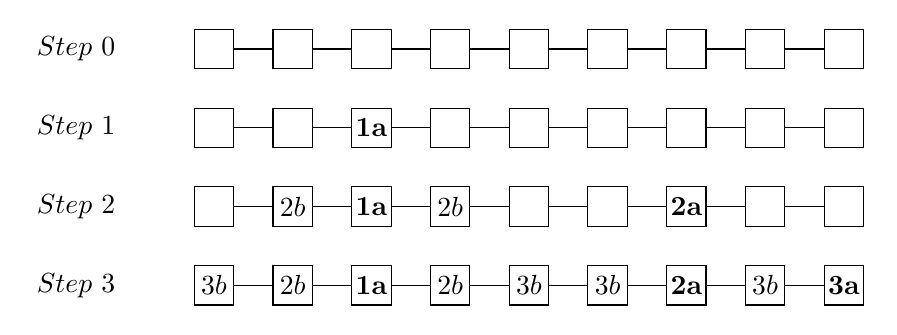
\begin{tikzpicture}
	    \draw (-4,0) rectangle (-3.5, 0.5);
	    \draw (-3,0) rectangle (-2.5, 0.5);\draw (-3.5,0.25) -- (-3, 0.25);
	    \draw (-2,0) rectangle (-1.5, 0.5);\draw (-2.5,0.25) -- (-2, 0.25);
	    \draw (-1,0) rectangle (-0.5, 0.5);\draw (-1.5,0.25) -- (-1, 0.25);
	    \draw (0,0) rectangle (0.5, 0.5);\draw (-0.5,0.25) -- (0, 0.25);
    	\draw (1,0) rectangle (1.5, 0.5);\draw (0.5,0.25) -- (1, 0.25);
	    \draw (2,0) rectangle (2.5, 0.5);\draw (1.5,0.25) -- (2, 0.25);
		\draw (3,0) rectangle (3.5, 0.5);\draw (2.5,0.25) -- (3, 0.25);
		\draw (4,0) rectangle (4.5, 0.5);\draw (3.5,0.25) -- (4, 0.25);
		
		\node at (-5.5,0.25) {$Step\ 3$};
    	\node at (-3.75,0.25) {$3b$};
    	\node at (-2.75,0.25) {$2b$};
		\node at (-1.75,0.25) {$\textbf{1a}$};
		\node at (-0.75,0.25) {$2b$};
		\node at (0.25,0.25) {$3b$};
    	\node at (1.25,0.25) {$3b$};
		\node at (2.25,0.25) {$\textbf{2a}$};
		\node at (3.25,0.25) {$3b$};
		\node at (4.25,0.25) {$\textbf{3a}$};
    	
		\draw (-4,1) rectangle (-3.5, 1.5);
		\draw (-3,1) rectangle (-2.5, 1.5);\draw (-3.5,1.25) -- (-3, 1.25);
    	\draw (-2,1) rectangle (-1.5, 1.5);\draw (-2.5,1.25) -- (-2, 1.25);
    	\draw (-1,1) rectangle (-0.5, 1.5);\draw (-1.5,1.25) -- (-1, 1.25);
    	\draw (0,1) rectangle (0.5, 1.5);\draw (-0.5,1.25) -- (0, 1.25);
    	\draw (1,1) rectangle (1.5, 1.5);\draw (0.5,1.25) -- (1, 1.25);
    	\draw (2,1) rectangle (2.5, 1.5);\draw (1.5,1.25) -- (2, 1.25);
		\draw (3,1) rectangle (3.5, 1.5);\draw (2.5,1.25) -- (3, 1.25);
		\draw (4,1) rectangle (4.5, 1.5);\draw (3.5,1.25) -- (4, 1.25);
		
		\node at (-5.5,1.25) {$Step\ 2$};
		\node at (-2.75,1.25) {$2b$};
		\node at (-1.75,1.25) {$\textbf{1a}$};
    	\node at (-0.75,1.25) {$2b$};
   		\node at (2.25,1.25) {$\textbf{2a}$};
		
		\draw (-4,2) rectangle (-3.5, 2.5);
		\draw (-3,2) rectangle (-2.5, 2.5);\draw (-3.5,2.25) -- (-3, 2.25);
		\draw (-2,2) rectangle (-1.5, 2.5);\draw (-2.5,2.25) -- (-2, 2.25);
		\draw (-1,2) rectangle (-0.5, 2.5);\draw (-1.5,2.25) -- (-1, 2.25);
		\draw (0,2) rectangle (0.5, 2.5);\draw (-0.5,2.25) -- (0, 2.25);
		\draw (1,2) rectangle (1.5, 2.5);\draw (0.5,2.25) -- (1, 2.25);
		\draw (2,2) rectangle (2.5, 2.5);\draw (1.5,2.25) -- (2, 2.25);
		\draw (3,2) rectangle (3.5, 2.5);\draw (2.5,2.25) -- (3, 2.25);
		\draw (4,2) rectangle (4.5, 2.5);\draw (3.5,2.25) -- (4, 2.25);
		
		\node at (-5.5,2.25) {$Step\ 1$};
		\node at (-1.75,2.25) {$\textbf{1a}$};
		
		\draw (-4,3) rectangle (-3.5, 3.5);
		\draw (-3,3) rectangle (-2.5, 3.5);\draw (-3.5,3.25) -- (-3, 3.25);
		\draw (-2,3) rectangle (-1.5, 3.5);\draw (-2.5,3.25) -- (-2, 3.25);
		\draw (-1,3) rectangle (-0.5, 3.5);\draw (-1.5,3.25) -- (-1, 3.25);
		\draw (0,3) rectangle (0.5, 3.5);\draw (-0.5,3.25) -- (0, 3.25);
    	\draw (1,3) rectangle (1.5, 3.5);\draw (0.5,3.25) -- (1, 3.25);
    	\draw (2,3) rectangle (2.5, 3.5);\draw (1.5,3.25) -- (2, 3.25);
    	\draw (3,3) rectangle (3.5, 3.5);\draw (2.5,3.25) -- (3, 3.25);
    	\draw (4,3) rectangle (4.5, 3.5);\draw (3.5,3.25) -- (4, 3.25);
    	    
	    \node at (-5.5,3.25) {$Step\ 0$};
    \end{tikzpicture}
	\caption{Burning of a path of $9$ vertices (optimal procedure). The vertices are marked by the step number in which they are burned. For each step, the vertex which is selected (arbitrarily) as a victim to be burned (the fire source) is marked by \textbf{\textit{a}}, and those which are burned by the fire spread from already burned vertices are marked by \textbf{\textit{b}}.}
	\label{figure:burn-path-9}
\end{figure}

\section{Optimal burning of some general graphs}\label{section:burn-general-graphs-optimally}

We start with defining isometric subgraph. An isometric subgraph of a graph is defined as follows.

\textbf{Isometric subgraph}\index{isometric subgraph}: A subgraph $H$ of a graph $G$ is called an \textit{isometric subgraph} if for every pair of nodes $u$ and $v$ in $H$, we have that the shortest distance between them in $H$ is equal to the shortest distance between them in $G$. If $G$ is a tree, and then we have that $H$ is an \textit{isometric tree}\index{isometric subtree} of $G$ is the same conditions satisfy.

It can be easily observed that any connected subgraph of a tree is its isometric subtree. Bonato et al. \cite{Bonato2016} have showed that if the burning number of a graph $G$ is $b(G)=k^\prime$, then the burning number of $H$, an isometric subtree of $G$ is $b(H)\leq b(G)=k^\prime$. We show this in \Cref{theorem:burn-isomorphic-subtree}.

\begin{theorem}\label{theorem:burn-isomorphic-subtree}
    Let that the burning number of a graph $G$ is $b(G)=k^\prime$, then the burning number of $H$, an isometric subtree of $G$ is $b(H)\leq b(G)=k^\prime$.
\end{theorem}

\begin{proof}
    Let for contradiction that $b(G)<b(H)$. Let the burning number of $H$ be $k^\prime$. From our assumption, we have that $b(G)\leq k^\prime-1$. This implies that there exists a burning sequence $S^\prime=(y_1,y_2,...,y_{k^\prime-1})$ which is able to burn $G$ completely.
    
    $H$ cannot be burned by any burning sequence of length less than $k^\prime$. It means that for any burning sequence of length less than $k^\prime$, at least one vertex in $H$ remains unburned. Since $H$ is an isometric subtree of $G$, we have that for any burning sequence of length less than $k^\prime$, at least one vertex in $G$ also remains unburned. So we need at least one more fire source in $S^\prime$ to burn $G$ which is a contradiction to our assumption.
\end{proof}

Similarly, we can obtain a proof that for any graph $G$, the burning number of an isometric subgraph of $G$ is not more then its own burning number $b(G)$. \Cref{theorem:burn-connected-graph-radius-r} and \Cref{theorem:burn-k-component-radius-r} we proved in \cite{Bonato2016}.

\begin{theorem}\label{theorem:burn-connected-graph-radius-r}
    If a connected graph $G$ is of radius $r$, then $b(G)\leq r+1$.
\end{theorem}

\begin{proof}
    Let $v$ be the vertex from which the distance of each vertex in $G.V$ is atmost $r$. Let that we have put a fire source on $v$ in the first time step. $\because G.N_{r}[v]=G.V$, $G$ will eventually get burnt within $r$ more time-steps irrespective of the position of the fire sources that are put in all other time-steps.
\end{proof}

\begin{theorem}\label{theorem:burn-k-component-radius-r}
    Let that $G$ is a graph containing $k$ connected components, each having a radius atmost $r$, then $b(G)\leq r+k$.
\end{theorem}

\begin{proof}
    Let there be $k$ components $C_1,C_2,\dots,C_k$ in a graph $G$, each of maximum radius $r$. Let $v_i$ be a vertex in $C_i$, $\forall\ 1\leq i\leq k$, such that it is atmost at a distance $r$ from all the other vertices in $C_i$.
    
    Let that in each time-step we put a fire source such that in step $i$, we put a fire source on $v_i$. Within next $r$ time-steps $G$ will be burnt.
\end{proof}

Next we discuss the burning procedure on some examples of spider graphs\index{burning spider graphs}. $SP(3,4)$ can be burnt optimally in 4 steps. As demonstrated in \Cref{figure:burn-SP34-optimal}, an optimal burning sequence of the presented graph $SP(3,\ 4)$ is $S^\prime_{SP(3,4)}=(b,\ h,\ l,\ m)$, which is of size $4$.

\begin{figure}
    \centering
    \subfigure[]{
        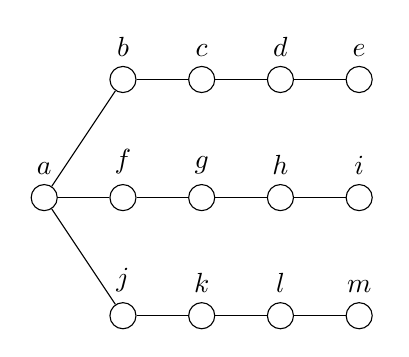
\begin{tikzpicture}
            \node[draw, shape=circle, label=above:{$a$}] (AA) at (0,0) {};
            
            \node[draw, shape=circle, label=above:{$b$}] (AB) at (1, 1.5) {};
            \node[draw, shape=circle, label=above:{$c$}] (AC) at (2, 1.5) {};
            \node[draw, shape=circle, label=above:{$d$}] (AD) at (3, 1.5) {};
            \node[draw, shape=circle, label=above:{$e$}] (AE) at (4, 1.5) {};
                
            \draw (AA) -- (AB);
            \draw (AB) -- (AC);
            \draw (AC) -- (AD);
            \draw (AD) -- (AE);
            
            \node[draw, shape=circle, label=above:{$f$}] (AB) at (1, 0) {};
            \node[draw, shape=circle, label=above:{$g$}] (AC) at (2, 0) {};
            \node[draw, shape=circle, label=above:{$h$}] (AD) at (3, 0) {};
            \node[draw, shape=circle, label=above:{$i$}] (AE) at (4, 0) {};
                
            \draw (AA) -- (AB);
            \draw (AB) -- (AC);
            \draw (AC) -- (AD);
            \draw (AD) -- (AE);
            
            \node[draw, shape=circle, label=above:{$j$}] (AB) at (1, -1.5) {};
            \node[draw, shape=circle, label=above:{$k$}] (AC) at (2, -1.5) {};
            \node[draw, shape=circle, label=above:{$l$}] (AD) at (3, -1.5) {};
            \node[draw, shape=circle, label=above:{$m$}] (AE) at (4, -1.5) {};
                
            \draw (AA) -- (AB);
            \draw (AB) -- (AC);
            \draw (AC) -- (AD);
            \draw (AD) -- (AE);
        \end{tikzpicture}
    }
    \subfigure[]{
        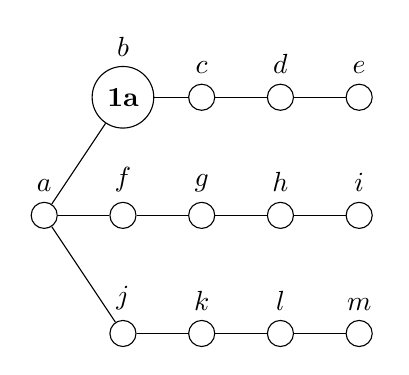
\begin{tikzpicture}
            \node[draw, shape=circle, label=above:{$a$}] (AA) at (0,0) {};
            
            \node[draw, shape=circle, label=above:{$b$}] (AB) at (1, 1.5) {\textbf{1a}};
            \node[draw, shape=circle, label=above:{$c$}] (AC) at (2, 1.5) {};
            \node[draw, shape=circle, label=above:{$d$}] (AD) at (3, 1.5) {};
            \node[draw, shape=circle, label=above:{$e$}] (AE) at (4, 1.5) {};
                
            \draw (AA) -- (AB);
            \draw (AB) -- (AC);
            \draw (AC) -- (AD);
            \draw (AD) -- (AE);
            
            \node[draw, shape=circle, label=above:{$f$}] (AB) at (1, 0) {};
            \node[draw, shape=circle, label=above:{$g$}] (AC) at (2, 0) {};
            \node[draw, shape=circle, label=above:{$h$}] (AD) at (3, 0) {};
            \node[draw, shape=circle, label=above:{$i$}] (AE) at (4, 0) {};
                
            \draw (AA) -- (AB);
            \draw (AB) -- (AC);
            \draw (AC) -- (AD);
            \draw (AD) -- (AE);
            
            \node[draw, shape=circle, label=above:{$j$}] (AB) at (1, -1.5) {};
            \node[draw, shape=circle, label=above:{$k$}] (AC) at (2, -1.5) {};
            \node[draw, shape=circle, label=above:{$l$}] (AD) at (3, -1.5) {};
            \node[draw, shape=circle, label=above:{$m$}] (AE) at (4, -1.5) {};
                
            \draw (AA) -- (AB);
            \draw (AB) -- (AC);
            \draw (AC) -- (AD);
            \draw (AD) -- (AE);
        \end{tikzpicture}
    }
    \subfigure[]{
        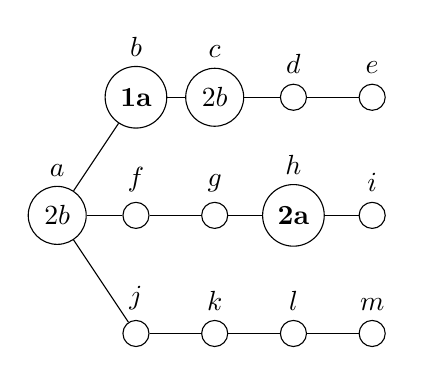
\begin{tikzpicture}
            \node[draw, shape=circle, label=above:{$a$}] (AA) at (0,0) {$2b$};
            
            \node[draw, shape=circle, label=above:{$b$}] (AB) at (1, 1.5) {\textbf{1a}};
            \node[draw, shape=circle, label=above:{$c$}] (AC) at (2, 1.5) {$2b$};
            \node[draw, shape=circle, label=above:{$d$}] (AD) at (3, 1.5) {};
            \node[draw, shape=circle, label=above:{$e$}] (AE) at (4, 1.5) {};
                
            \draw (AA) -- (AB);
            \draw (AB) -- (AC);
            \draw (AC) -- (AD);
            \draw (AD) -- (AE);
            
            \node[draw, shape=circle, label=above:{$f$}] (AB) at (1, 0) {};
            \node[draw, shape=circle, label=above:{$g$}] (AC) at (2, 0) {};
            \node[draw, shape=circle, label=above:{$h$}] (AD) at (3, 0) {\textbf{2a}};
            \node[draw, shape=circle, label=above:{$i$}] (AE) at (4, 0) {};
                
            \draw (AA) -- (AB);
            \draw (AB) -- (AC);
            \draw (AC) -- (AD);
            \draw (AD) -- (AE);
            
            \node[draw, shape=circle, label=above:{$j$}] (AB) at (1, -1.5) {};
            \node[draw, shape=circle, label=above:{$k$}] (AC) at (2, -1.5) {};
            \node[draw, shape=circle, label=above:{$l$}] (AD) at (3, -1.5) {};
            \node[draw, shape=circle, label=above:{$m$}] (AE) at (4, -1.5) {};
                
            \draw (AA) -- (AB);
            \draw (AB) -- (AC);
            \draw (AC) -- (AD);
            \draw (AD) -- (AE);
        \end{tikzpicture}
    }
    \subfigure[]{
        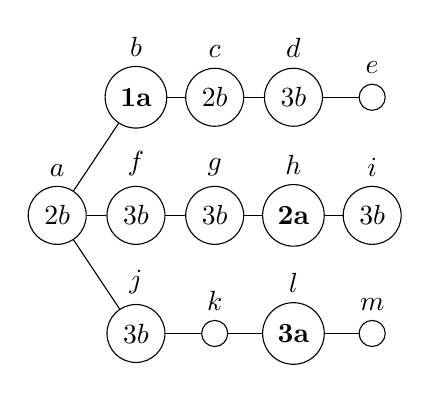
\begin{tikzpicture}
            \node[draw, shape=circle, label=above:{$a$}] (AA) at (0,0) {$2b$};
            
            \node[draw, shape=circle, label=above:{$b$}] (AB) at (1, 1.5) {\textbf{1a}};
            \node[draw, shape=circle, label=above:{$c$}] (AC) at (2, 1.5) {$2b$};
            \node[draw, shape=circle, label=above:{$d$}] (AD) at (3, 1.5) {$3b$};
            \node[draw, shape=circle, label=above:{$e$}] (AE) at (4, 1.5) {};
                
            \draw (AA) -- (AB);
            \draw (AB) -- (AC);
            \draw (AC) -- (AD);
            \draw (AD) -- (AE);
            
            \node[draw, shape=circle, label=above:{$f$}] (AB) at (1, 0) {$3b$};
            \node[draw, shape=circle, label=above:{$g$}] (AC) at (2, 0) {$3b$};
            \node[draw, shape=circle, label=above:{$h$}] (AD) at (3, 0) {\textbf{2a}};
            \node[draw, shape=circle, label=above:{$i$}] (AE) at (4, 0) {$3b$};
                
            \draw (AA) -- (AB);
            \draw (AB) -- (AC);
            \draw (AC) -- (AD);
            \draw (AD) -- (AE);
            
            \node[draw, shape=circle, label=above:{$j$}] (AB) at (1, -1.5) {$3b$};
            \node[draw, shape=circle, label=above:{$k$}] (AC) at (2, -1.5) {};
            \node[draw, shape=circle, label=above:{$l$}] (AD) at (3, -1.5) {\textbf{3a}};
            \node[draw, shape=circle, label=above:{$m$}] (AE) at (4, -1.5) {};
                
            \draw (AA) -- (AB);
            \draw (AB) -- (AC);
            \draw (AC) -- (AD);
            \draw (AD) -- (AE);
        \end{tikzpicture}
    }
    \subfigure[]{
        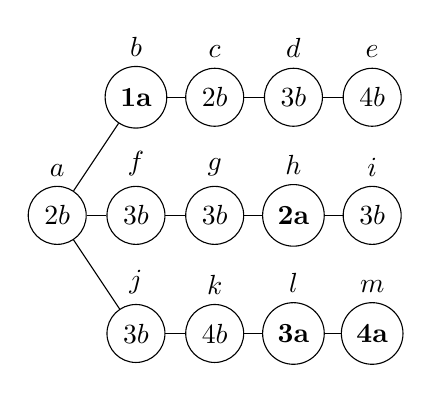
\begin{tikzpicture}
            \node[draw, shape=circle, label=above:{$a$}] (AA) at (0,0) {$2b$};
            
            \node[draw, shape=circle, label=above:{$b$}] (AB) at (1, 1.5) {\textbf{1a}};
            \node[draw, shape=circle, label=above:{$c$}] (AC) at (2, 1.5) {$2b$};
            \node[draw, shape=circle, label=above:{$d$}] (AD) at (3, 1.5) {$3b$};
            \node[draw, shape=circle, label=above:{$e$}] (AE) at (4, 1.5) {$4b$};
                
            \draw (AA) -- (AB);
            \draw (AB) -- (AC);
            \draw (AC) -- (AD);
            \draw (AD) -- (AE);
            
            \node[draw, shape=circle, label=above:{$f$}] (AB) at (1, 0) {$3b$};
            \node[draw, shape=circle, label=above:{$g$}] (AC) at (2, 0) {$3b$};
            \node[draw, shape=circle, label=above:{$h$}] (AD) at (3, 0) {\textbf{2a}};
            \node[draw, shape=circle, label=above:{$i$}] (AE) at (4, 0) {$3b$};
                
            \draw (AA) -- (AB);
            \draw (AB) -- (AC);
            \draw (AC) -- (AD);
            \draw (AD) -- (AE);
            
            \node[draw, shape=circle, label=above:{$j$}] (AB) at (1, -1.5) {$3b$};
            \node[draw, shape=circle, label=above:{$k$}] (AC) at (2, -1.5) {$4b$};
            \node[draw, shape=circle, label=above:{$l$}] (AD) at (3, -1.5) {\textbf{3a}};
            \node[draw, shape=circle, label=above:{$m$}] (AE) at (4, -1.5) {\textbf{4a}};
                
            \draw (AA) -- (AB);
            \draw (AB) -- (AC);
            \draw (AC) -- (AD);
            \draw (AD) -- (AE);
        \end{tikzpicture}
    }
    \caption{Optimal burning of $SP(3,\ 4)$.}
    \label{figure:burn-SP34-optimal}
\end{figure}

If we increase one more arm in $SP(3,\ 4)$, it becomes $SP(4,\ 4)$, and now we need at least $5$ time steps to burn it; a burnt $SP(4,\ 4)$ is shown in figure \Cref{figure:burn-SP44-optimal}. An optimal burning sequence of the presented graph $SP(4,4)$ is $S^\prime_{SP(4,4)}=(b,\ h,\ l,\ m,\ q)$.

\begin{figure}
    \centering
    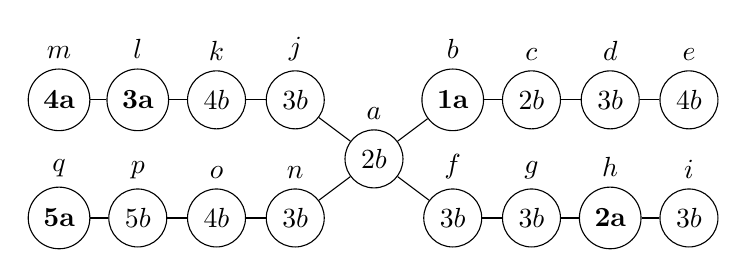
\begin{tikzpicture}
        \node[draw, shape=circle, label=above:{$a$}] (AA) at (0,0) {$2b$};
        
        \node[draw, shape=circle, label=above:{$b$}] (AB) at (1, .75) {\textbf{1a}};
        \node[draw, shape=circle, label=above:{$c$}] (AC) at (2, .75) {$2b$};
        \node[draw, shape=circle, label=above:{$d$}] (AD) at (3, .75) {$3b$};
        \node[draw, shape=circle, label=above:{$e$}] (AE) at (4, .75) {$4b$};
            
        \draw (AA) -- (AB);
        \draw (AB) -- (AC);
        \draw (AC) -- (AD);
        \draw (AD) -- (AE);
        
        \node[draw, shape=circle, label=above:{$f$}] (AB) at (1, -.75) {$3b$};
        \node[draw, shape=circle, label=above:{$g$}] (AC) at (2, -.75) {$3b$};
        \node[draw, shape=circle, label=above:{$h$}] (AD) at (3, -.75) {\textbf{2a}};
        \node[draw, shape=circle, label=above:{$i$}] (AE) at (4, -.75) {$3b$};
            
        \draw (AA) -- (AB);
        \draw (AB) -- (AC);
        \draw (AC) -- (AD);
        \draw (AD) -- (AE);
        
        \node[draw, shape=circle, label=above:{$j$}] (AB) at (-1, .75) {$3b$};
        \node[draw, shape=circle, label=above:{$k$}] (AC) at (-2, .75) {$4b$};
        \node[draw, shape=circle, label=above:{$l$}] (AD) at (-3, .75) {\textbf{3a}};
        \node[draw, shape=circle, label=above:{$m$}] (AE) at (-4, .75) {\textbf{4a}};
        
        \draw (AA) -- (AB);
        \draw (AB) -- (AC);
        \draw (AC) -- (AD);
        \draw (AD) -- (AE);
            
        \node[draw, shape=circle, label=above:{$n$}] (AB) at (-1, -.75) {$3b$};
        \node[draw, shape=circle, label=above:{$o$}] (AC) at (-2, -.75) {$4b$};
        \node[draw, shape=circle, label=above:{$p$}] (AD) at (-3, -.75) {$5b$};
        \node[draw, shape=circle, label=above:{$q$}] (AE) at (-4, -.75) {\textbf{5a}};
        
        \draw (AA) -- (AB);
        \draw (AB) -- (AC);
        \draw (AC) -- (AD);
        \draw (AD) -- (AE);
    \end{tikzpicture}
    \caption{Optimal burning of $SP(4,\ 4)$}
    \label{figure:burn-SP44-optimal}
\end{figure}

Bessy et al \cite{Bessy2017} have proved that for a graph $SP(s,\ r)$ if $s \geq r$, then $b(SP(s,\ r))$ $=$ $r+1$, and if $s \geq r+2$, then it is necessary for any optimal burning sequence to have first fire source on the spider head. We show this as \Cref{lemma:b(SP)}. \Cref{figure:burn-1-component} is an example of this phenomenon; it shows burning of $SP(d,\ k^\prime-1)$, where $d \geq k^\prime+1$. In its optimal burning sequence $S^\prime_{SP(d,k^\prime-1)} = (y_1, y_2, y_3, . . ., y_{k^\prime})$, the first fire source $y_1$ is placed on the spider head.

\begin{lemma}\label{lemma:b(SP)}
    For a graph $SP(s,\ r)$ if $s \geq r$, then $b(SP(s,\ r))$ $=$ $r+1$, and if $s \geq r+2$, then it is necessary for any optimal burning sequence to have first fire source on the spider head.
\end{lemma}

\begin{proof}
    We start with discussing a spider graph $SP(r,r)$ whose number of arms $r$ is equal to the length of each arm. The radius of $SP(r,r)$ is $r$. So by \Cref{theorem:burn-connected-graph-radius-r} we have that $b(SP(r,r))\leq r+1$.
    
    Now we show that $b(SP(r,r))\geq r+1$.
    Let for contradiction that $b(SP(r,r))\leq r$. This implies that there is a w-burning sequence $S^\prime=(x_1,x_2,...,x_{k^\prime})$ such that $k^\prime\leq r$ which is able to burn $SP(s,r)$. No fire source in $S^\prime$ shall be able to burn more than one leaf node in $G$ because the distance between any two leaf nodes is $2r$. We will be able to burn atmost $k^\prime \leq r$ leaf nodes in $k^\prime$ rounds. This implies that at least $1$ leaf node will be left unburned. This implies that $S^\prime$ must contain at least one more fire source which is a contradiction.
    
    Thus, $b(SP(r,r))=r+1$.
    
    Given that $s \geq r+2$, by \Cref{theorem:burn-isomorphic-subtree} $b(SP(s,\ r))\geq r+1$. Also since the radius of $SP(s,r)$ is of radius $r$, we have that $SP(s,r)\leq r+1$. So we have that $SP(s,r)=r+1$.
    
    Next we show that if $s \geq r+2$, then it is necessary for any optimal burning sequence to have first fire source on the spider head. Let that an optimal burning sequence $S^\prime=(y_1,y_2,...,y_{r+1})$ of length $r+1$ is able to burn $SP(s,r)$. Let for contradiction that the first fire source is not placed at the spider head. So we have that at least $r+1$ leaf nodes cannot be burned by $y_1$. Also, no other fire source will be able to burn two leaf nodes simultaneously because the distance between any two leaf nodes is $2r$. So we have that the fire sources $y_2,...,y_{r+1}$ will be able to burn at most $r$ leaf nodes. We have that at least one leaf node will remain unburned which is a contradiction. So the first fire source $y_1\in S^\prime$ must be placed at the spider head. This concludes the proof.
\end{proof}

\begin{figure}
	\centering
	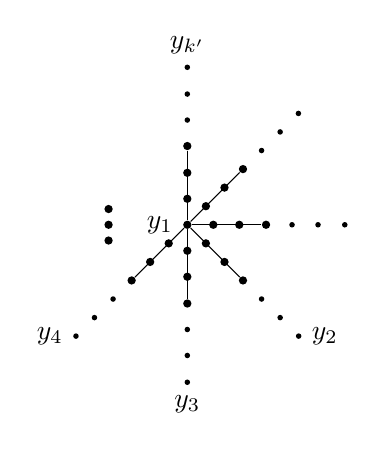
\begin{tikzpicture}
	    \node [circle, fill=black, inner sep=0pt, minimum size=3pt, label=left:{$y_1$}] (AA) at (0,0) {};
	    
	    \node [circle, fill=black, inner sep=0pt, minimum size=3pt] at (0,.33) {};
	    \node [circle, fill=black, inner sep=0pt, minimum size=3pt] at (.236,.236) {};
	    \node [circle, fill=black, inner sep=0pt, minimum size=3pt] at (.33,0) {};
	    \node [circle, fill=black, inner sep=0pt, minimum size=3pt] at (.236,-.236) {};
	    \node [circle, fill=black, inner sep=0pt, minimum size=3pt] at (0,-.33) {};
	    \node [circle, fill=black, inner sep=0pt, minimum size=3pt] at (-.236,-.236) {};
	    
	    \node [circle, fill=black, inner sep=0pt, minimum size=3pt] at (0,.66) {};
	    \node [circle, fill=black, inner sep=0pt, minimum size=3pt] at (.472,.472) {};
	    \node [circle, fill=black, inner sep=0pt, minimum size=3pt] at (.66,0) {};
	    \node [circle, fill=black, inner sep=0pt, minimum size=3pt] at (.472,-.472) {};
	    \node [circle, fill=black, inner sep=0pt, minimum size=3pt] at (0,-.66) {};
	    \node [circle, fill=black, inner sep=0pt, minimum size=3pt] at (-.472,-.472) {};
	    
	    \node [circle, fill=black, inner sep=0pt, minimum size=3pt] (AB) at (0,1) {};
	    \node [circle, fill=black, inner sep=0pt, minimum size=3pt] (AC) at (.707,.707) {};
	    \node [circle, fill=black, inner sep=0pt, minimum size=3pt] (AD) at (1,0) {};
	    \node [circle, fill=black, inner sep=0pt, minimum size=3pt] (AE) at (.707,-.707) {};
	    \node [circle, fill=black, inner sep=0pt, minimum size=3pt] (AF) at (0,-1) {};
	    \node [circle, fill=black, inner sep=0pt, minimum size=3pt] (AG) at (-.707,-.707) {};
	    
	    \node [circle, fill=black, inner sep=0pt, minimum size=2pt] at (0,1.33) {};
	    \node [circle, fill=black, inner sep=0pt, minimum size=2pt] at (.707+.236,.707+.236) {};
	    \node [circle, fill=black, inner sep=0pt, minimum size=2pt] at (1.33,0) {};
	    \node [circle, fill=black, inner sep=0pt, minimum size=2pt] at (.707+.236,-.707-.236) {};
	    \node [circle, fill=black, inner sep=0pt, minimum size=2pt] at (0,-1.33) {};
	    \node [circle, fill=black, inner sep=0pt, minimum size=2pt] at (-.707-.236,-.707-.236) {};
	    
	    \node [circle, fill=black, inner sep=0pt, minimum size=2pt] at (0,1.66) {};
	    \node [circle, fill=black, inner sep=0pt, minimum size=2pt] at (.707+.472,.707+.472) {};
	    \node [circle, fill=black, inner sep=0pt, minimum size=2pt] at (1.66,0) {};
	    \node [circle, fill=black, inner sep=0pt, minimum size=2pt] at (.707+.472,-.707-.472) {};
	    \node [circle, fill=black, inner sep=0pt, minimum size=2pt] at (0,-1.66) {};
	    \node [circle, fill=black, inner sep=0pt, minimum size=2pt] at (-.707-.472,-.707-.472) {};
	    
	    \node [circle, fill=black, inner sep=0pt, minimum size=2pt, label=above:{$y_{k^{\prime}}$}] at (0,2) {};
	    \node [circle, fill=black, inner sep=0pt, minimum size=2pt] at (1.411,1.414) {};
	    \node [circle, fill=black, inner sep=0pt, minimum size=2pt] at (2,0) {};
	    \node [circle, fill=black, inner sep=0pt, minimum size=2pt, label=right:{$y_2$}] at (1.414,-1.414) {};
	    \node [circle, fill=black, inner sep=0pt, minimum size=2pt, label=below:{$y_3$}] at (0,-2) {};
	    \node [circle, fill=black, inner sep=0pt, minimum size=2pt, label=left:{$y_4$}] at (-1.414,-1.414) {};
	    
	    \node [circle, fill=black, inner sep=0pt, minimum size=3pt] at (-1,0) {};
	    \node [circle, fill=black, inner sep=0pt, minimum size=3pt] at (-1,-0.2) {};
	    \node [circle, fill=black, inner sep=0pt, minimum size=3pt] at (-1,0.2) {};
	    
		\draw (AA) -- (AB);
		\draw (AA) -- (AC);
		\draw (AA) -- (AD);
		\draw (AA) -- (AE);
		\draw (AA) -- (AF);
		\draw (AA) -- (AG);
		
	\end{tikzpicture}
	\caption{Optimal burning of a graph $SP(d,\ k^\prime-1)$, where $d \geq k^\prime+1$. $S^\prime_{SP(d,k^\prime-1)} = (y_1, y_2, . . ., y_{k^{\prime}})$ is the optimal burning sequence.}
	\label{figure:burn-1-component}
\end{figure}

\Cref{figure:burn-1-component} shows burning of a graph containing only one connected component, whereas \Cref{figure:burn-many-components} represents the burning of a graph $G_{SP}$ which is a disjoint union of $k^{\prime}$ components\index{burning (example) graph containing more than one components}. Each component $comp_i: 1\leq i\leq k^\prime$ is a spider graph where $comp_i = SP(d_i, i-1),\ d_i \geq i+1$. This implies the graph $G_{SP} = SP(d_1,\ 0)$ $\cup$ $SP(d_2,\ 1)$ $\cup$ $SP(d_3,\ 2)$ $\cup$ $. . .$ $\cup$ $SP(d_{k^\prime},\ k^\prime-1)$.

The burning number of both the graphs $SP(d,\ k^\prime-1)$ and $G_{SP}$ is $k^{\prime}$. It can be easily observed \cite{Bonato2016} that if an arbitrary graph $G^\prime$ contains $k$ connected components, then the burning number of this graph, $b(G^\prime) \geq k$.

\begin{figure}
	\begin{minipage}{1\textwidth}
		\centering
		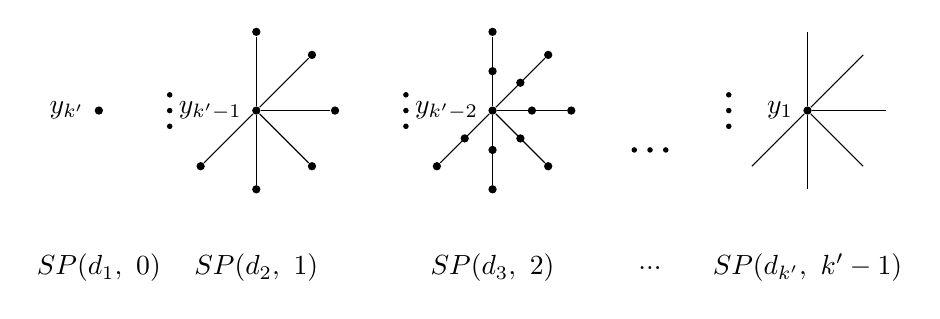
\begin{tikzpicture}
		    \node [circle, fill=black, inner sep=0pt, minimum size=3pt, label=left:{$y_{k^{\prime}}$}] at (-2,0) {};
		    
		    
		    \node [circle, fill=black, inner sep=0pt, minimum size=3pt, label=left:{$y_{k^{\prime}-1}$}] (AA) at (0,0) {};
		    \node [circle, fill=black, inner sep=0pt, minimum size=3pt] (AB) at (0,1) {};
		    \node [circle, fill=black, inner sep=0pt, minimum size=3pt] (AC) at (0.707,0.707) {};
		    \node [circle, fill=black, inner sep=0pt, minimum size=3pt] (AD) at (1,0) {};
		    \node [circle, fill=black, inner sep=0pt, minimum size=3pt] (AE) at (0.707,-0.707) {};
		    \node [circle, fill=black, inner sep=0pt, minimum size=3pt] (AF) at (0,-1) {};
		    \node [circle, fill=black, inner sep=0pt, minimum size=3pt] (AG) at (-0.707,-0.707) {};
		    
		    \node [circle, fill=black, inner sep=0pt, minimum size=2pt] at (-1.1,0) {};
		    \node [circle, fill=black, inner sep=0pt, minimum size=2pt] at (-1.1,-0.2) {};
		    \node [circle, fill=black, inner sep=0pt, minimum size=2pt] at (-1.1,0.2) {};
		    
			\draw (AA) -- (AB);
			\draw (AA) -- (AC);
			\draw (AA) -- (AD);
			\draw (AA) -- (AE);
			\draw (AA) -- (AF);
			\draw (AA) -- (AG);
			
			
		    \node [circle, fill=black, inner sep=0pt, minimum size=3pt, label=left:{$y_{k^{\prime}-2}$}] (BA) at (3,0) {};
		    \node [circle, fill=black, inner sep=0pt, minimum size=3pt] (BB) at (3,0.5) {};
		    \node [circle, fill=black, inner sep=0pt, minimum size=3pt] (BC) at (3,1) {};
		    \node [circle, fill=black, inner sep=0pt, minimum size=3pt] (BD) at (3.3535,0.3535) {};
		    \node [circle, fill=black, inner sep=0pt, minimum size=3pt] (BE) at (3.707,0.707) {};
		    \node [circle, fill=black, inner sep=0pt, minimum size=3pt] (BF) at (3.5,0) {};
		    \node [circle, fill=black, inner sep=0pt, minimum size=3pt] (BG) at (3+1,0) {};
		    \node [circle, fill=black, inner sep=0pt, minimum size=3pt] (BH) at (3.3535,-0.3535) {};
		    \node [circle, fill=black, inner sep=0pt, minimum size=3pt] (BI) at (3.707,-0.707) {};
		    \node [circle, fill=black, inner sep=0pt, minimum size=3pt] (BJ) at (3,-0.5) {};
		    \node [circle, fill=black, inner sep=0pt, minimum size=3pt] (BK) at (3,-1) {};
		    \node [circle, fill=black, inner sep=0pt, minimum size=3pt] (BL) at (3-0.3535,-0.3535) {};
		    \node [circle, fill=black, inner sep=0pt, minimum size=3pt] (BM) at (3-0.707,-0.707) {};
		    
		    \node [circle, fill=black, inner sep=0pt, minimum size=2pt] at (3-1.1,0) {};
		    \node [circle, fill=black, inner sep=0pt, minimum size=2pt] at (3-1.1,-0.2) {};
		    \node [circle, fill=black, inner sep=0pt, minimum size=2pt] at (3-1.1,0.2) {};
		    
			\draw (BA) -- (BC);
			\draw (BA) -- (BE);
			\draw (BA) -- (BG);
			\draw (BA) -- (BI);
			\draw (BA) -- (BK);
			\draw (BA) -- (BM);
			
			
			\node [circle, fill=black, inner sep=0pt, minimum size=2pt] at (5,-.5) {};
		    \node [circle, fill=black, inner sep=0pt, minimum size=2pt] at (5.2,-.5) {};
		    \node [circle, fill=black, inner sep=0pt, minimum size=2pt] at (5-0.2,-.5) {};
			
			
		    \node [circle, fill=black, inner sep=0pt, minimum size=3pt, label=left:{$y_1$}] (CA) at (7,0) {};
		    
		    \node [circle, fill=black, inner sep=0pt, minimum size=2pt] at (7-1,0) {};
		    \node [circle, fill=black, inner sep=0pt, minimum size=2pt] at (7-1,-0.2) {};
		    \node [circle, fill=black, inner sep=0pt, minimum size=2pt] at (7-1,0.2) {};
		    
			\draw (CA) -- (7,1);
			\draw (CA) -- (7.707,0.707);
			\draw (CA) -- (7+1,0);
			\draw (CA) -- (7.707,-0.707);
			\draw (CA) -- (7,-1);
			\draw (CA) -- (7-0.707,-0.707);
			
			
			\node at (-2,-2) {$SP(d_1,\ 0)$};
			\node at (0,-2) {$SP(d_2,\ 1)$};
			\node at (3,-2) {$SP(d_3,\ 2)$};
			\node at (5,-2) {$. . .$};
			\node at (7,-2) {$SP(d_{k^\prime},\ k^\prime-1)$};
		\end{tikzpicture}
	\end{minipage}
	
	\caption{Optimal burning of a graph $G_{SP}$ with $k^\prime$ connected components, where $G_{SP} = SP(d_1,\ 0)$ $\cup$ $SP(d_2,\ 1)$ $\cup$ $SP(d_3,\ 2)$ $\cup$ $. . .$ $\cup$ $SP(d_{k^\prime},\ k^\prime-1)$ and $d_i \geq i+1$.}
	\label{figure:burn-many-components}
\end{figure}

\section{Algorithm for burning general graphs optimally}

\index{algorithm: optimal burning of general graphs}An algorithm to compute a burning sequence for an arbitrary graph is given in \cite{Bessy2017}. \Cref{algorithm:burn-general-optimal} is similar to that algorithm; it computes an optimal burning sequence for an arbitrary input graph $G$ in exponential time. It is a brute force algorithm which checks for every possible permutation of vertices in $G$, sequentially, if it is a valid burning sequence.\\

\begin{algorithm}\label{algorithm:burn-general-optimal}
Given the input graph $G$ perform the following steps.
\end{algorithm}

\textbf{\textit{Stage 1.}} $n = |G.V|$. Let that the vertices in $G.V$ be labelled as $v_1,v_2,\dots,v_n$. $i=1$. if $i\leq n$, perform the following steps.

\textbf{\textit{Stage 1.1.}} For every permutation $P$ of size $i$ in the sequence $(1,2,\dots,n)$ (where $P$ itself is a sequence of numbers), perform the following steps.

\textbf{\textit{Stage 1.1.2.}} Let $S = (v_{P[1]},v_{P[2]},\dots,v_{P[|P|]})$. If $S$ is able to burn $G$, that is, if $(G,S)$ is passed as input to \Cref{algorithm:burn-verify}, it returns $true$, then return $S$.

\textbf{\textit{Stage 1.2.}} $i=i+1$.

% \bibliography{ref.bib}
% \bibliographystyle{plain}